\documentclass{article}

\usepackage[letterpaper]{geometry}
\usepackage{siunitx}
\usepackage{amsmath}
\usepackage{graphicx}
\usepackage{amssymb}

\title{4125 HW 2}
\author{Duncan Wilkie}
\date{3 February 2022}

\begin{document}

\maketitle

\section*{1.34a}
For process A, the volume is constant, so there is no work done on the gas. Therefore, $\Delta U=-Q$. There are five degrees of freedom, all quadratic, for a diatomic molecule with frozen-out vibrational modes; the internal energy is therefore $\frac{5}{2}kT_i$ at the beginning of the process and $\frac{5}{2}kT_f$ at the end. The delta is then, applying the equation of state,
\[\Delta U=\frac{5}{2}k(T_f-T_i)=\frac{5}{2}\left(P_fV_f-P_iV_i \right)=\frac{5}{2}(P_2V_1-P_1V_1)\]
The heat put into the gas is then $Q=\frac{5}{2}(P_2V_1-P_1V_1)$.

For process B, the pressure is constant, so the work done by the gas is the integral $W=-\int PdV$. Since the process is a horizontal line on the $PV$ diagram, this is just the area of the rectangle, i.e. $W=-P(V_f-V_i)=P_2(V_1-V_2)$. The internal energy is the same as above, so the change in it is
\[\Delta U=\frac{5}{2}k(T_f-T_i)=\frac{5}{2}(P_2V_2-P_2V_1)\]
The heat put in the gas is therefore \[Q=\Delta U-W=\frac{5P}{2}(V_f-V_i)-(-P(V_f-V_i))=\frac{7}{2}P_2(V_2-V_1)\]

Processes C and D have the same formulas in terms of initial and final varaibles as processes A and B, just with different values for those variables.
For process C,
\[W=0\textrm{, } \Delta U=\frac{5}{2}(P_1V_2-P_2V_2)\textrm{, } Q=\frac{5}{2}(P_1V_2-P_2V_2)\]
For process D,
\[W=P_1(V_2-V_1)\textrm{, }\Delta U=\frac{5}{2}(P_1V_1-P_1V_2)\textrm{, }Q=\frac{7}{2}P_1(V_1-V_2)\]

\section*{1.34b}
During step A, heat is added to the gas and the piston is held fixed. During step B, the piston is pulled back and heat added so the pressure remains constant. During step C, the piston is held fixed and heat is removed. During step D, the piston is pushed in and heat removed from the gas so the pressure remains constant.

\section*{1.34c}
These net values are just the sums of their values in each case, i.e.
\[W=W_A+W_B+W_C+W_D=0+P_2(V_1-V_2)+0+P_1(V_2-V_1)=-(P_2-P_1)(V_2-V_1)\]
\[\Delta U=\Delta U_A+\Delta U_B+\Delta U_C+\Delta U_D=\frac{5}{2}(P_2V_1-P_1V_1)+\frac{5}{2}(P_2V_2-P_2V_1)+\frac{5}{2}(P_1V_2-P_2V_2)+\frac{5}{2}(P_1V_1-P_1V_2)\]
\[=0\]
\[Q=Q_A+Q_B+Q_C+Q_D=\frac{5}{2}(P_2V_1-P_1V_1)+\frac{7}{2}(P_2V_2-P_2V_1)+\frac{5}{2}(P_1V_2-P_2V_2)+\frac{7}{2}(P_1V_1-P_1V_2)\]
\[=P_1V_1-P_2V_1+P_2V_2-P_1V_2=(P_2-P_1)(V_2-V_1)\]

\section*{1.38}
The process for bubble A is adiabatic, and so satisfies $V=\left( \frac{P_0V_0}{P} \right)^{1/\gamma}$. The process for bubble B is isothermal, and so satisfies $V=\frac{P_0V_0}{P}$. Since $\gamma=1+\frac{2}{f}$, $\gamma > 1$, so an adiabatic process increases in volume faster than an isotherm as pressure increases. In other words, if an adiabat and an isotherm share the same starting point and pressure decreases, the adiabat will have a greater volume for the same pressure, implying bubble A will be larger at the surface of the lake. A plot of the two $V(P)$ curves with $P_0V_0=1$ and $f=5\Leftrightarrow \gamma=\frac{5}{3}$ appears below for illustration.
\[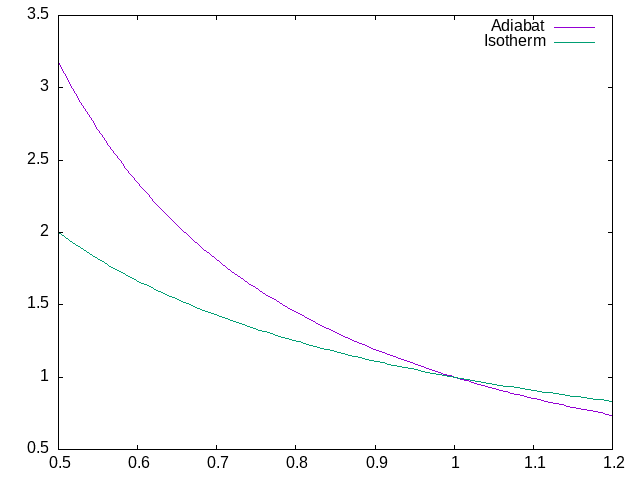
\includegraphics[scale=0.75]{138.png}\]

\section*{1.40a}
The equation of state yields the following expression for temperature:
\[T=\frac{PV}{k}\]
Applying the equation for an adiabat
\[PV^{1+2/f}=P_0V_0\Leftrightarrow V=\left( \frac{P_0V_0}{P} \right)^\frac{1}{1+2/f}\]
we may eliminate V in the equation of state to obtain
\[T(P)=\frac{(P_0V_0)^{1/(1+2/f)}}{kP^{\frac{1}{1+2/f}-1}}\]
Differentiating with respect to $P$,
\[\frac{dT}{dP}=\left( 1-\frac{1}{1+2/f} \right)\frac{(P_0V_0)^{1/(1+2/f)}}{kP^{\frac{1}{1+2/f}-1}P}=\frac{2/f}{1+2/f}\frac{T}{P}=\frac{2}{f+2}\frac{T}{P}\]
as desired.

\section*{1.40b}
Using the chain rule $\frac{dT}{dz}=\frac{dT}{dP}\frac{dP}{dz}$, the temperature gradient is
\[\frac{dT}{dz}=-\frac{2}{f+2}\frac{T}{P}\frac{mg}{kT}P=-\frac{2mg}{k(f+2)}\]

\section*{1.43}
The specific heat of water at constant volume was given in the book as $\SI{4.2}{J/g^\circ C }$. The atomic mass of a water molecule is \SI{18}{amu}, so about 18 grams of water corresponds to one mole. The heat capacity per molecule is then
\[\frac{C}{N}\frac{(\SI{18}{g})(\SI{4.2}{J/g^\circ C})}{\SI{6.02e23}{}}=\SI{1.26e-22}{J/^\circ C}=9.1k\]
The equipartition theorem suggests that, presuming all degrees of freedom are quadratic, this number is equal to $\frac{f}{2}k$, since multiplying by the total number of particles and a temperature would yield the internal energy of the water. This suggests the water molecule has around 18 degrees of freedom, which seems a little absurd.

\section*{1.48}
The power density actually absorbed by the snow pack is $0.1(\SI{1}{kW/m^2})=\SI{100}{W/m^2}$. In a square meter of the snow pack, there is a total volume of $\SI{2}{m^3}$. Half of this is ice, so one cubic meter of ice is present. The density of ice is $\SI{919}{kg/m^3}$ according to a table I found online. If the ice is already at \SI{32}{^\circ C}, the amount of energy required to melt it using the latent heat of fusion given in the book of $\SI{333}{J/g}=\SI{333}{kJ}{kg}$ is
\[Q=Lm={(\SI{333}{kJ/kg})}{(\SI{919}{kg/m^3})}=\SI{306}{MJ}\]
Dividing this by the power the snow absorbs, it would take
\[t=\frac{Q}{P}=\frac{\SI{306e6}{J}}{\SI{}}\]



\end{document}
%%% Local Variables:
%%% mode: latex
%%% TeX-master: t
%%% End:
